\part{Basic mechanics}
\frame{\partpage}

\begin{frame}{Point masses}
	\begin{itemize}
		\pause\item For now we assume everything is a \textbf{point mass},
			i.e.\ ignore the actual shape and size of objects
		\pause\item \textbf{Mass} is measured in \textbf{kilograms}
		\pause\item Not to be confused with \textbf{weight} (GCSE physics!)
	\end{itemize}
\end{frame}

\begin{frame}{Position, velocity and acceleration}
	\begin{itemize}
		\pause\item \textbf{Position} describes an object's location in space
			\begin{itemize}
				\pause\item Usually expressed as a 3-vector relative to the \textbf{origin}
				\pause\item Measured in \textbf{metres}
			\end{itemize}
		\pause\item \textbf{Velocity} is \textbf{rate of change of position}
			\begin{itemize}
				\pause\item Measured in \textbf{metres per second} (ms$^{-1}$)
				\pause\item Velocity is a \textbf{vector}
				\pause\item Speed is a \textbf{scalar} (a number), the magnitude of velocity
				\pause\item speed : velocity :: distance : position
			\end{itemize}
		\pause\item \textbf{Acceleration} is \textbf{rate of change of velocity}
			\begin{itemize}
				\pause\item Measured in \textbf{metres per second per second} (ms$^{-2}$)
			\end{itemize}
	\end{itemize}
\end{frame}

\begin{frame}{Newton's Laws of Motion}
	\begin{center}
		\pause An object remains at rest or moves at constant velocity unless acted upon by an external force
		
		\vspace{2ex}
		
		\pause $F = ma$: The sum of forces acting upon an object is equal to its mass multiplied by its acceleration
		
		\vspace{2ex}
		
		\pause When one body exerts a force on another, the second body exerts an equal and opposite force on the first
	\end{center}
\end{frame}

\begin{frame}{Force}
	\begin{itemize}
		\pause\item Measured in \textbf{Newtons} (N)
		\pause\item $F = ma$: 1N of force causes a 1kg object to accelerate by 1ms$^{-2}$
		\pause\item Forces occur when objects \textbf{interact}
		\pause\item E.g.\ gravity, air resistance, friction
		\pause\item E.g.\ reaction force: stops objects from passing through each other
		\pause\item E.g.\ applied forces: car engine, rocket engine, launched projectile, human muscle, ...
	\end{itemize}
\end{frame}

\begin{frame}{Simulating Newtonian physics}
	\begin{itemize}
		\pause\item Each object needs to store its \textbf{position} and \textbf{velocity}
		\pause\item On each frame:
			\begin{itemize}
				\pause\item Apply \textbf{numerical integration} to determine the new position from the current velocity
				\pause\item Calculate the \textbf{forces} acting upon the object and use these to calculate \textbf{acceleration}
					$$ F = ma \quad \implies \quad a = \frac{F}{m} $$
				\pause\item Apply \textbf{numerical integration} again to determine the new velocity from the current acceleration
			\end{itemize}
	\end{itemize}
\end{frame}

\begin{frame}{Gravity}
	\begin{itemize}
		\pause\item Gravity pulls \textbf{all objects} with mass \textbf{towards each other}
		\pause\item Gravitational force is tiny unless one or both objects has a huge mass (e.g.\ a planet...)
		\pause\item Near the surface of a planet, gravity pulls objects \textbf{downwards} (i.e.\ towards the centre of the planet)
			with a force called \textbf{weight}
		\pause\item $w=mg$, where $w$ is weight, $m$ is mass and $g$ is the \textbf{gravitational constant}
		\pause\item On Earth, $g \approx 9.81$ (often rounded to $g = 10$)
	\end{itemize}
\end{frame}

\begin{frame}{Gravity}
	\begin{align*}
		F &= ma \\
		F &= w = mg \\
		\implies mg &= ma \\
		\implies g &= a
	\end{align*}
	\begin{itemize}
		\pause\item So gravity applies \textbf{the same} acceleration (9.81 ms$^{-2}$ downwards) to all objects \textbf{regardless} of weight!
		\pause\item Famous experiment: in a \textbf{vacuum} (no air resistance), a bowling ball falls at the \textbf{same speed} as a feather
	\end{itemize}
\end{frame}

\begin{frame}{Basic collision response}
	\begin{columns}
		\begin{column}{0.4\textwidth}
			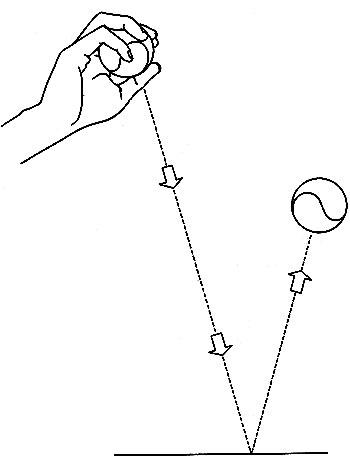
\includegraphics[width=\textwidth]{bounce_reflection}
		\end{column}
		\begin{column}{0.58\textwidth}
			\begin{itemize}
				\pause\item For an \textbf{elastic collision}, the component of velocity parallel to the \textbf{surface normal}
					is \textbf{reversed}
				\pause\item E.g.\ if the surface is the $xz$ plane, flip the $y$ component
				\pause\item For an \textbf{inelastic collision}, some velocity is lost
				\pause\item Flip the $y$ component and multiply it by something between $0$ and $1$
			\end{itemize}
		\end{column}
	\end{columns}
\end{frame}

